%%
%% This is file `sample-sigconf-biblatex.tex',
%% generated with the docstrip utility.
%%
%% The original source files were:
%%
%% samples.dtx  (with options: `sigconf-biblatex')
%% 
%% IMPORTANT NOTICE:
%% 
%% For the copyright see the source file.
%% 
%% Any modified versions of this file must be 
%% with new filenames distinct from sample-sigconf-biblatex.tex.
%% 
%% For distribution of the original source see the terms
%% for copying and modification in the file samples.dtx.
%% 
%% This generated file may be distributed as long as the
%% original source files, as listed above, are part of the
%% same distribution. (The sources need not necessarily be
%% in the same archive or directory.)
%%
%%
%% Commands for TeXCount
%TC:macro \cite [option:text,text]
%TC:macro \citep [option:text,text]
%TC:macro \citet [option:text,text]
%TC:envir table 0 1
%TC:envir table* 0 1
%TC:envir tabular [ignore] word
%TC:envir displaymath 0 word
%TC:envir math 0 word
%TC:envir comment 0 0
%%
%%
%% The first command in your LaTeX source must be the \documentclass
%% command.
%%
%% For submission and review of your manuscript please change the
%% command to \documentclass[manuscript, screen, review]{acmart}.
%%
%% When submitting camera ready or to TAPS, please change the command
%% to \documentclass[sigconf]{acmart} or whichever template is required
%% for your publication.
%%
%%
\documentclass[sigconf]{acmart}
%\documentclass[sigplan,10pt]{acmart}

%% \BibTeX command to typeset BibTeX logo in the docs
\AtBeginDocument{%
	\providecommand\BibTeX{{%
			Bib\TeX}}}

\usepackage{graphicx}
\usepackage{algorithm}
\usepackage{algpseudocode}
\usepackage{booktabs} 
\usepackage{threeparttable}
\usepackage{multirow}
\usepackage{enumitem}
\usepackage{colortbl}
\usepackage[most]{tcolorbox}
\usepackage{caption}
\usepackage{balance}
\usepackage[normalem]{ulem}
\usepackage{xcolor}
\pagestyle{empty}


\usepackage{pifont}
\usepackage{booktabs}
\usepackage{cleveref}
\crefname{section}{§}{§§}
\Crefname{section}{§}{§§}

\newcommand{\mytodoblue}[1]{\textcolor{blue}{\ding{46}~{\sf}~#1}}
\newcommand{\mytodored}[1]{\textcolor{red}{\ding{46}~{\sf}~#1}}
\newcommand{\mytodogreen}[1]{\textcolor{mygreen}{\ding{46}~{\sf}~#1}}
\newcommand{\mytodoorange}[1]{\textcolor{orange}{\ding{46}~{\sf}~#1}}
\newcommand{\mytodocyan}[1]{\textcolor{cyan}{\ding{46}~{\sf}~#1}}
\newcommand{\mytodopink}[1]{\textcolor{purple}{\ding{46}~{\sf}~#1}}
\usepackage{pgffor}
\usepackage{pifont} % For checkmark and cross symbols

\usepackage{xcolor,pifont}
\usepackage{amsmath}
%\usepackage{algorithm}
%\usepackage{algpseudocode}


% 自定义彩色打勾和打叉命令
\newcommand{\cmark}{\textcolor{green!60!black}{\ding{51}}}   % 绿色打勾
\newcommand{\xmark}{\textcolor{red}{\ding{55}}}   % 红色打叉

% 定义 Definition 环境
\theoremstyle{definition}
\newtheorem{definition}{Definition}[section]
\newtheorem{example}{Example}[section]


% to show s or not
\newif\ifshowcomments
%\showcommentsfalse
\showcommentstrue
\ifshowcomments
\newcommand{\wu}[1]{\mytodored{[wu: #1]}}
\newcommand{\cp}[1]{\mytodored{[cp: #1]}}
%\newcommand{\zhang}[1]{\mytodoorange{[zhang: #1]}}
\newcommand{\lin}[1]{\mytodored{[lin: #1]}}
%\newcommand{\other}[1]{\mytodoblue{[other: #1]}}
\else
\newcommand{\wu}[1]{}
\newcommand{\cp}[1]{}
%\newcommand{\zhang}[1]{}
\newcommand{\lin}[1]{}
%\newcommand{\other}[1]{}
\fi

\newif\ifshowrevisioncomments
\showcommentsfalse
%\showrevisioncommentstrue
\showrevisioncommentsfalse
\ifshowrevisioncomments
\newcommand{\revision}[1]{\textcolor{blue}{{#1}}}
\newcommand{\deletion}[1]{\textcolor{red}{{\sout{#1}}}}
\else
\newcommand{\revision}[1]{#1}
\newcommand{\deletion}[1]{}
\fi


\newcommand{\toolname}{\textsc{DMLScope}}
\newcommand{\model}{\textsc{ASRMT}}
\newcommand{\reported}{44}
\newcommand{\confirmed}{42}
\newcommand{\fixed}{9}
\newcommand{\pending}{2}

\bibliographystyle{ACM-Reference-Format}

\settopmatter{printacmref=false}
\settopmatter{printfolios=true}
\setcopyright{none}
\renewcommand\footnotetextcopyrightpermission[1]{}
\pagestyle{plain}

%\settopmatter{printfolios=true}
%\pagestyle{plain}

% 改成数字引用
\citestyle{acmnumeric}
\begin{document}
\newtcolorbox{mybox}[2][]{
  colframe = black,
  colback  = gray!20,
  coltitle = black,
  left = 1mm,
  right = 1mm,
  top = 1mm,
  bottom = 1mm,
  boxsep=5pt,
  arc=2mm,
  title=#2,
  #1
}

\title{DMLScope: Uncovering Logical Bugs in Database DML via Approximate State-Relation–Driven Metamorphic Testing}


\begin{abstract}
	Database Management Systems (DBMSs) are critical infrastructure for modern data-driven applications, and logical bugs in DBMSs may silently produce incorrect query results or corrupted database states. 
	While prior work has made significant progress in detecting logical bugs in read-only queries, considerably less attention has been paid to state-modifying SQL statements. 
	Data manipulation language (DML) statements such as \texttt{INSERT}, \texttt{UPDATE}, and \texttt{DELETE} directly modify persistent database contents, making their correctness harder to validate and their consequences more severe. 
	
	In this paper, we propose \textit{Approximate State-Relation--Driven Metamorphic Testing} (ASRMT), a novel testing paradigm for detecting logical bugs in state-modifying SQL statements. 
	ASRMT characterizes DML semantics through state effects, an abstract and comparable representation of the state changes induced by DML execution, and validates correctness by checking approximate relations between the effects of related statements. 
	Based on this paradigm, we develop \toolname, which systematically generates executable DML statements, synthesizes approximate variants, executes them from the same database pre-state, and verifies whether their state effects satisfy the expected approximate relations. 
	We evaluate \toolname\ on six widely used DBMSs and uncover 51 previously unknown bugs, including 25 logical bugs. 
	The results show that \toolname\ effectively detects logical bugs in DML statements and substantially broadens the scope of DBMS testing beyond existing techniques.
\end{abstract}



\settopmatter{printfolios=true}
\maketitle
\pagestyle{plain}
\section{Introduction}
\label{sec:intro}


%\begin{figure}[t]
%	\centering
%	%	\vspace{-3mm}
%	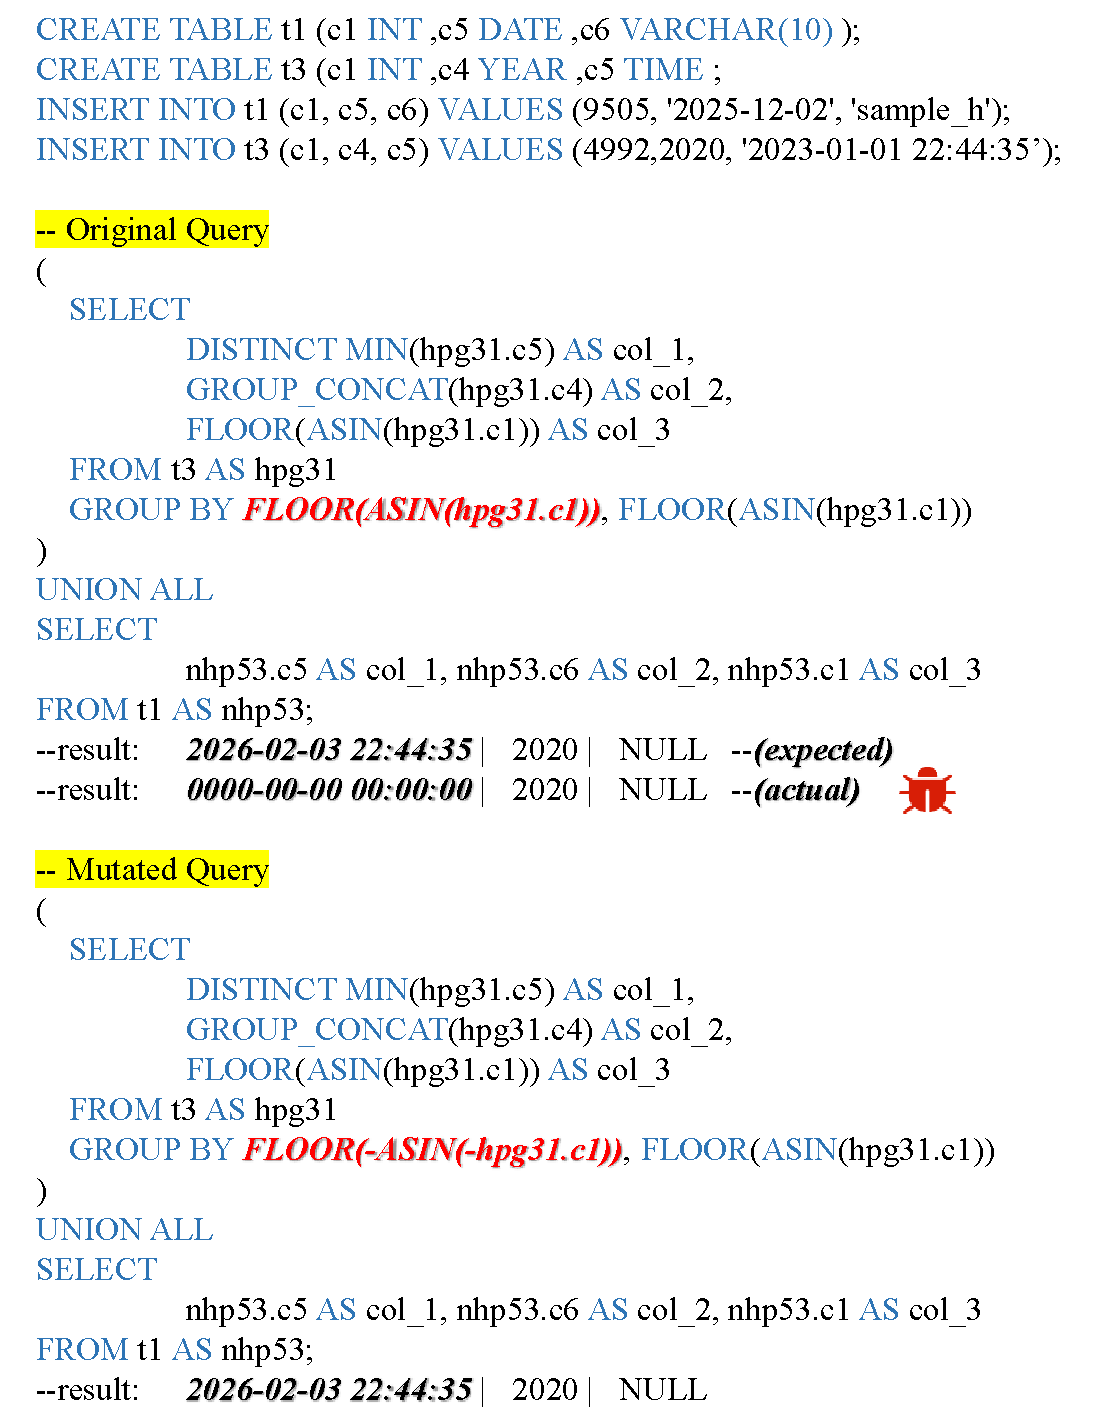
\includegraphics[width=1\linewidth]{./images/motivating_example.pdf} 
%	\vspace{-6mm}
%	\caption{\textbf{Queries exposing a logical bug in a built-in SQL function in Percona Server.}}
%	\label{fig:motivating example}
%	\vspace{-5mm}
%\end{figure}


% Contribution
%Overall, we make the following contributions:
%\begin{itemize}[leftmargin=10pt]
%	\item We propose a novel methodology \textit{Function Property--Driven Metamorphic Testing} for systematically detecting logical bugs in built-in SQL functions.
%	\item We implement \toolname\ as a DBMS testing tool, which automatically generates, mutates, and verifies SQL queries based on \textit{Function Property--Driven Metamorphic Testing}, enabling the detection of logical bugs in SQL functions.
%	\item We evaluate \toolname\ on six real-world DBMSs and find \reported\ previously unknown logical bugs.  
%	To further facilitate research on DBMS testing, we open-source \toolname\ at \url{https://anonymous.4open.science/status/FPMT-DBTesting-D3CA}.
%\end{itemize}







\section{Background and Motivation}
\label{sec:background and motivation}

% Background

% Challenges 生成复杂的DML
% Challenges 缺乏有效的测试预言机

% Solution 1:
% Solution 2： 受到 Pinolo 的启发

% Motivating Example
\section{Approach}
\label{sec:approach}

% 可以按照 Pinolo 的写法来
\subsection{Other Implementation Details}
\label{subsec:Implementation}

We implemented \toolname\ as a prototype DBMS testing system in Python, consisting of \textcolor{red}{13,455} lines of code.
To support mutation at the structural level, \toolname\ leverages \textsc{SQLGlot}~\cite{tobymao_sqlglot} to parse original DML statements into ASTs, enabling precise application of approximate mutators while preserving syntactic and semantic correctness.
During testing, \toolname\ executes generated statements on target DBMSs and collects execution results for further analysis.
To improve the usability of detected bugs, we adopt \textsc{SQLess}~\cite{lin2024sqless} to simplify failing cases and isolate their root causes, and further apply a deduplication strategy following \textsc{Pinolo}~\cite{hao2023pinolo} to eliminate redundant bug reports.
\toolname\ is primarily designed for MySQL-compatible systems, including TiDB and OceanBase, but its modular architecture allows for straightforward adaptation to other DBMS dialects by customizing syntax- and type-related components.
In practice, such adaptation requires only lightweight modifications, and can be further automated using tools such as \textsc{QTRAN}~\cite{lin2025qtran}, which facilitates cross-dialect deployment of metamorphic testing techniques.
\section{Evaluation}
\label{sec: Evaluation}

%Our evaluation aims to answer the following questions to demonstrate the effectiveness of \toolname :
%
%\begin{itemize}[leftmargin=20pt]
%	\item[\textbf{\textit{Q1}}] How many unique and new bugs in real-world DBMSs can \toolname\ detect? (Section~\ref{sec:eval-bugs})
%%	\item[\textbf{\textit{Q2}}] How diverse are the logical bugs found by \toolname? (Section~\ref{sec:eval-diversity})
%	\item[\textbf{\textit{Q2}}] Can \toolname\ find logical bugs that are missed by existing approaches? (Section~\ref{sec:eval-compare})
%\end{itemize}

\subsection{Experimental Setup}
\textbf{Tested DBMS.}
We evaluate \toolname\ on 6 widely used DBMSs, as summarized in Table~\ref{table:testdbms}. 
These DBMSs were chosen based on their popularity and extensive use in real-world applications. 
%MySQL and MariaDB are long-established and widely deployed relational DBMSs, while Percona represents an industrial MySQL-derived system. 
%TiDB is a modern distributed SQL database, and DuckDB and MonetDB are widely recognized analytical DBMSs with strong influence in modern data processing workloads. 
All of these DBMSs have undergone extensive testing for both logical~\cite{hao2023pinolo,kamm2023testing,rigger2020testing,lin2025qtran,rigger2020detecting,rigger2020finding,song2023testing,tang2023detecting,jiang2024detecting,deng2025detecting,zhang2025constant} and crash bugs~\cite{jiang2023dynsql,sqlsmith,pingcap_gorandgen_2022,zhong2020squirrel}.
Although finding new bugs in such widely tested systems is challenging, it serves to validate the effectiveness of \toolname. 
In our experiments, \toolname\ tests the latest versions of each DBMS.  
We run \toolname\ on each DBMS for 24 hours.


\begin{table}[h]
	\centering
	\caption{\textbf{The demographics of the DBMSs under test}}
	\label{table:testdbms}
	\small
	\vspace{-2mm}
	\resizebox{\dimexpr\textwidth/2\relax}{!}{
		\begin{tabular}{lcccc}
			\toprule
			\textbf{DBMS}       & \textbf{Version}           & \textbf{GitHub Stars} & \textbf{DB-Engine}         & \textbf{First Release} \\ 
			\midrule
			MySQL~\cite{mysql}      & 9.5.0             & 11.9K        & 2                 & 1995          \\
			MariaDB~\cite{mariadb}    & 12.2.2 & 6.7K        & 13                & 2009          \\
			MonetDB~\cite{monetdb}  & 11.55.3 & 458 & 150  & 2004          \\
			Percona~\cite{percona}      & 8.0.43-34       & 1.2K         & 122               & 2008          \\
			DuckDB~\cite{duckdb}    & 1.5.0  & 37.3K    & 43               & 2018          \\
			TiDB~\cite{tidb}       & 8.5.5 & 39.4K        & 85                & 2016          \\
			\bottomrule
		\end{tabular}
	}
	\vspace{-2mm}
\end{table}

\textbf{Environment}. 
We conduct the experiments on one server with 104-cores Intel(R) Xeon(R) Gold 6230R CPU @2.10GHz and 500 GB memory. 
The server operates under the Ubuntu 20.04 OS, with the 5.4.0-135-generic version of the Linux kernel.

\subsection{Bug Detection}
\label{sec:eval-bugs}

Table~\ref{tab:bug_summary} summarizes the unique bugs found by \toolname\ across six DBMSs. 
Overall, \toolname\ detected 21 logical bugs, 8 abnormal errors, and 18 crashes, yielding 47 unique bugs in total. 
The logical bugs are distributed across all tested systems, including 5 in MySQL, 3 in MariaDB, 5 in MonetDB, 5 in Percona, 1 in DuckDB, and 2 in TiDB. 
Among all reported bugs, 47 have been confirmed by developers, and 27 have already been fixed. 
These results show that \toolname\ can effectively uncover severe correctness issues even in mature and extensively tested DBMSs.

\begin{table}[t]
	\centering
	\caption{\toolname\ founded 45 unique bugs in six DBMSs.}
	\vspace{-2mm}
	\label{tab:bug_summary}
	\resizebox{\columnwidth}{!}{
		\begin{tabular}{lcccccc}
			\toprule
			\multirow{2}{*}{\textbf{DBMS}} & \multicolumn{3}{c}{\textbf{Bug type}} & \multicolumn{2}{c}{\textbf{Bug status}} \\
			\cmidrule(lr){2-4} \cmidrule(lr){5-6}
			& \textbf{Logical bug} & \textbf{Abnormal error} & \textbf{Crash} & \textbf{Confirmed} & \textbf{Fixed} \\
			\midrule
			MySQL      & 5 & 0 & 3 & 8 & 0 \\
			MariaDB       & 3 & 0 & 0 & 3  & 0 \\
			MonetDB & 5 & 8 & 12 & 25 & 25 \\
			Percona      & 5 & 0 & 1 & 6 & 0 \\
			DuckDB      & 1 & 0 & 2 & 3 & 2 \\
			TiDB        & 2 & 0 & 0 & 2  & 0 \\
			\midrule
			Total       & 21 & 8 & 18 & 47 & 27 \\
			\bottomrule
		\end{tabular}
	}
	\vspace{-3mm}
\end{table}
    
\textbf{Bug Importance.}
Although anecdotal, developer feedback is an important indicator of an approach’s effectiveness and the significance of the bugs found. 
Two DBMS companies reached out to us regarding our testing efforts; both were interested in how we discovered the bugs, and one even invited us to help them find more. 
For example, a developer from PolarDB commented: ``Outstanding work, this tool looks very useful, and we will fully support any technical requirements you may need."
Additionally, we received positive feedback on public bug tracking platforms. 
Among the confirmed bugs, all reported bugs in MariaDB were labeled as ``Major,'' representing the highest severity level, while two bugs in MySQL and two bugs in Percona were classified as ``Serious,'' indicating their significant impact.

\textbf{Throughput.}
We evaluate the efficiency of our test generation by measuring the number of test cases produced per second, where each test case consists of an original DML statement and its corresponding approximate variant. 
Specifically, \toolname\ generates \textcolor{red}{xxx} test cases/sec for MySQL, \textcolor{red}{xxx} for MariaDB, \textcolor{red}{xxx} for MonetDB, \textcolor{red}{xxx} for Percona, \textcolor{red}{xxx} for DuckDB, and \textcolor{red}{xxx} for TiDB. 
Beyond competitive throughput, \toolname\ also attains high execution success rates on most DBMSs, reaching \textcolor{red}{xxx}\% for MySQL, \textcolor{red}{xxx}\% for MariaDB, \textcolor{red}{xxx}\% for MonetDB, \textcolor{red}{xxx}\% for Percona, \textcolor{red}{xxx}\% for DuckDB, and \textcolor{red}{xxx}\% for TiDB.
We further measure the average complexity of generated statements using their size in bytes. 
The average statement size is \textcolor{red}{xxx} bytes for MySQL, \textcolor{red}{xxx} for MariaDB, \textcolor{red}{xxx} for MonetDB, \textcolor{red}{xxx} for Percona, \textcolor{red}{xxx} for DuckDB, and \textcolor{red}{xxx} for TiDB. 
These results show that our structure-guided and constraint-aware generation strategy can efficiently produce a large volume of complex yet executable DML statements.

% Query Generation  （参考 Dinkel）
	% Query Validity (和 DQE 相比)
    % Throughput
    
%\subsection{Comprehensive Bug Analysis}
%\label{sec:eval-diversity}

\textbf{Bug Diversity.}
We analyze the 21 confirmed logical bugs from two perspectives: the diversity of DML types and the structural complexity of the triggering statements. 
In terms of DML types, the majority of bugs are caused by \texttt{UPDATE} statements (16/21), while the remaining involve \texttt{DELETE} (4/21) and \texttt{INSERT} (1/21), indicating that value-modifying operations are particularly error-prone. 
From a structural perspective, most bugs are triggered by complex query constructs: 18 out of 21 bugs involve subqueries, 8 involve joins, 10 involve set operations, and 14 involve logical predicates. 
These results show that DML logical bugs are highly correlated with rich query contexts and interactions among multiple SQL operators, rather than simple statements. 
Such complexity poses a significant challenge to existing approaches like \textsc{DQE}, which are limited to relatively simple and aligned query patterns and cannot effectively support complex constructs such as nested subqueries and set operations. 
In contrast, \toolname\ can systematically generate structurally rich DML statements and leverage state-relation-based oracles to robustly reason about their effects, enabling the detection of these complex and previously overlooked logical bugs.

\begin{table}[t]
	\centering
	\caption{\textbf{Feature distribution of detected DML logical bugs.}}
	\vspace{-2mm}
	\label{tab:bug_pattern}
	\resizebox{\columnwidth}{!}{
		\begin{tabular}{ccccccc}
			\toprule
			\textbf{ID} & \textbf{Bug ID} & \textbf{Type} & \textbf{Subquery} & \textbf{Join} & \textbf{SetOp} & \textbf{LogicOp} \\
			\midrule
			
			1  & \texttt{MySQL\#120047} & UPDATE & \cmark & \cmark & \xmark & \cmark \\
			2  & \texttt{MySQL\#120056} & UPDATE & \cmark & \cmark & \xmark & \cmark \\
			3  & \texttt{MySQL\#120057} & UPDATE & \cmark & \cmark & \cmark & \cmark \\
			4  & \texttt{MySQL\#120058} & UPDATE & \xmark & \cmark & \xmark & \cmark \\
			5  & \texttt{MySQL\#120203} & UPDATE & \cmark & \xmark & \xmark & \xmark \\
			
			6  & \texttt{MariaDB\#39065} & DELETE & \cmark & \xmark & \cmark & \xmark \\
			7  & \texttt{MariaDB\#39097} & UPDATE & \cmark & \xmark & \xmark & \cmark \\
			8  & \texttt{MariaDB\#39144} & UPDATE & \cmark & \xmark & \cmark & \cmark \\
			
			9  & \texttt{MonetDB\#7891} & UPDATE & \cmark & \xmark & \xmark & \cmark \\
			10 & \texttt{MonetDB\#7888} & UPDATE & \xmark & \xmark & \xmark & \cmark \\
			11 & \texttt{MonetDB\#7889} & DELETE & \cmark & \xmark & \cmark & \xmark \\
			12 & \texttt{MonetDB\#7890} & INSERT & \cmark & \xmark & \cmark & \cmark \\
			13 & \texttt{MonetDB\#7897} & DELETE & \cmark & \xmark & \cmark & \cmark \\
			
			14 & \texttt{Percona\#10877} & UPDATE & \cmark & \cmark & \xmark & \cmark \\
			15 & \texttt{Percona\#10878} & UPDATE & \cmark & \cmark & \xmark & \cmark \\
			16 & \texttt{Percona\#10879} & UPDATE & \cmark & \cmark & \cmark & \cmark \\
			17 & \texttt{Percona\#10906} & UPDATE & \xmark & \cmark & \xmark & \cmark \\
			18 & \texttt{Percona\#11008} & UPDATE & \cmark & \xmark & \xmark & \xmark \\
			
			19 & \texttt{DuckDB\#21609} & INSERT & \cmark & \cmark & \xmark & \cmark \\
			
			20 & \texttt{TiDB\#67018} & UPDATE & \cmark & \xmark & \cmark & \xmark \\
			21 & \texttt{TiDB\#67019} & DELETE & \cmark & \xmark & \cmark & \cmark \\
			
			\bottomrule
		\end{tabular}
	}
	\vspace{-3mm}
\end{table}

\textbf{Case Study.}

% RQ3：Comoporehensive Bug Analysis
	% Bug Statements：Update、Delete、Insert (Rules) 一个大表  id，bug id，type，（rule），EET的feature
% Selected Bugs
%   Update 、 Delete 、 Insert 各一个

\subsection{Comparative Study}
\label{sec:eval-compare}
To demonstrate that \toolname\ can detect DML logical bugs missed by existing methods, we conduct our comparative study from two perspectives: tool level and oracle level. 
At the tool level, we compare \toolname\ with six representative logical bug detection approaches, including \textsc{PQS}~\cite{rigger2020testing}, \textsc{NoREC}~\cite{rigger2020detecting}, \textsc{TLP}~\cite{rigger2020finding}, \textsc{DQE}~\cite{song2023testing}, \textsc{Pinolo}~\cite{hao2023pinolo}, and \textsc{EET}~\cite{jiang2024detecting}, by running each tool on the latest version of each supported DBMS for 24 hours. 
Since the baseline methods do not support all DBMSs tested by \toolname, the comparison is restricted to the DBMSs commonly supported by \toolname\ and each baseline method. 
As shown in Table~\ref{tab:tool-support-dbms}, \toolname\ consistently outperforms the baselines in terms of triggered logical bugs, finding 5, 3, 1, 10, 7, and 4 more bugs than \textsc{PQS}, \textsc{NoREC}, \textsc{TLP}, \textsc{DQE}, \textsc{Pinolo}, and \textsc{EET}, respectively, where each increment is computed only on the commonly supported DBMSs. Overall, \toolname\ triggers 21 logical bugs within 24 hours, whereas all baseline tools together trigger only 6.
At the oracle level, we analyze whether existing testing oracles are capable of detecting the logical bugs uncovered by \toolname. 
From a theoretical perspective, the \logical\ logical bugs detected by \toolname\ fundamentally rely on reasoning about state transitions, including which rows are affected and how their values are modified. 
However, existing query-centric approaches, such as \textsc{PQS}, \textsc{NoREC}, \textsc{TLP}, \textsc{Pinolo}, and \textsc{EET}, define correctness over returned query results and therefore cannot capture errors that only manifest in persistent state changes. 
Although \textsc{DQE} targets DML statements, its oracle is based on cross-statement row-access consistency and mainly checks whether related statements access the same tuples, making it insufficient for detecting value-level errors and many complex state transitions induced by joins, subqueries, and other rich DML constructs. 
As a result, the logical bugs detected by \toolname\ are not observable under the oracles used by these baseline approaches. 
This explains why the \logical\ logical bugs detected by \toolname\ are entirely disjoint from the 6 logical bugs triggered by the baselines, and highlights that \toolname\ explores a different and previously untested space of DML correctness. 
%At the oracle level, we further analyze why \toolname\ can uncover bugs missed by existing tools.  
%The \logical\ logical bugs detected by \toolname\ are entirely disjoint from the 6 logical bugs triggered by the baselines, indicating that \toolname\ discovers a different class of DML bugs. 
%This advantage stems from its stronger oracle design. 
%Existing query-centric approaches, such as \textsc{PQS}, \textsc{NoREC}, \textsc{TLP}, \textsc{Pinolo}, and \textsc{EET}, define correctness over returned query results and therefore are not naturally suited for reasoning about persistent state changes caused by DML execution, while \textsc{DQE} relies on cross-statement row-access consistency and mainly checks whether related statements touch the same tuples. 
%As a result, these approaches cannot naturally validate many value-level errors and complex state transitions induced by joins, subqueries, and other rich DML constructs. 
%In contrast, \toolname\ reasons directly about DML semantics through state effects and checks approximate relations over state changes, enabling it to detect logical bugs that are invisible to result-set-based or row-access-based oracles.
%These results show that \toolname\ not only outperforms existing methods in practice, but also complements them by exposing previously overlooked DML logical bugs.

%To compare \toolname\ against state-of-the-art DBMS testing methods, we selected six representative logical bug detection approaches for comparison: \textsc{PQS}~\cite{rigger2020testing}, \textsc{NoREC}~\cite{rigger2020detecting}, \textsc{TLP}~\cite{rigger2020finding}, \textsc{DQE}~\cite{song2023testing}, \textsc{Pinolo}~\cite{hao2023pinolo}, and \textsc{EET}~\cite{jiang2024detecting}. 
%We ran each tool on the latest version of each supported DBMS for 24 hours. 
%Since the baseline methods do not support all DBMSs tested by \toolname, the comparison is restricted to the DBMSs commonly supported by \toolname\ and each baseline method. 
%As shown in Table~\ref{tab:tool-support-dbms}, \toolname\ consistently outperforms the other tools in detecting logical bugs across the evaluated DBMSs. 
%Specifically, \toolname\ found 5, 3, 1, 10, 7, and 4 more bugs than \textsc{PQS}, \textsc{NoREC}, \textsc{TLP}, \textsc{DQE}, \textsc{Pinolo}, and \textsc{EET}, respectively. 
%Note that these increments are computed only on the DBMSs commonly supported by both approaches. 
%We further analyzed the relation between the bugs detected by existing tools and those detected by \toolname\ to examine whether \toolname\ can uncover bugs missed by prior methods. 
%Our results show that the \reported\ logical bugs detected by \toolname\ are entirely disjoint from the 6 logical bugs triggered by the baseline tools, indicating that \toolname\ can discover previously missed bugs and effectively complements existing methods.

\begin{table}[t]
	\centering
	\vspace{-2mm}
	\caption{\textbf{Number of logical bugs triggered in 24 hours.}}
	\vspace{-2mm}
	\small
	\label{tab:tool-support-dbms}
	\resizebox{\columnwidth}{!}{
		\begin{tabular}{l|ccccccc}
			\toprule
			\textbf{DBMS} & \textbf{PQS} & \textbf{NoREC} & \textbf{TLP} & \textbf{DQE} & \textbf{Pinolo} & \textbf{EET} & \textbf{\toolname} \\
			\midrule
			MySQL    & 0 & - & 4 & 0 & 2 & 3 & 5 \\
			MariaDB  & - & 0 & - & 0 & 1 & - & 3 \\
			MonetDB  & - & - & - & - & - & - & 5 \\
			Percona  & - & - & - & - & - & - & 5 \\
			DuckDB   & - & - & - & - & - & - & 1 \\
			TiDB     & - & - & 2 & 0 & 0 & 0 & 2 \\
			\midrule
			\textbf{Total}     & 0 & 0 & 6 & 0 & 3 & 3 & 21 \\
			\textbf{Increment} & 5 & 3 & 1 & 10 & 7 & 4 &  \\
			\bottomrule
		\end{tabular}
	}
	\raggedright
	\noindent \textbf{Note.} ``-'' indicates that the tool does not support the DBMS. \\
	``Increment'' is computed on the commonly supported DBMSs between the baseline tool and \toolname.
	\vspace{-5mm}
\end{table}

%\textbf{Temporal Comparison.}
%We also present a temporal comparison to evaluate whether \toolname\ can uncover DML logical bugs that have long existed but were missed by prior approaches. 
%For each confirmed logical bug discovered by \toolname, we trace its earliest bug-involved version and compare it against the publication timeline of existing DBMS testing approaches~\cite{rigger2020detecting,rigger2020finding,rigger2020testing,song2023testing,tang2023detecting,jiang2024detecting,song2024detecting,hao2023pinolo,deng2025detecting,ba2024keep}. 
%If a bug had already existed before the release of prior techniques but remained undiscovered until \toolname, we regard it as evidence that previous approaches failed to detect it. 
%This comparison is reasonable for two reasons. 
%First, the bugs reported by \toolname\ were not marked as duplicates by the corresponding developers, indicating that they had not been previously reported. 
%Second, most of the evaluated DBMSs have already been extensively tested by existing approaches, yet these long-lived DML bugs still remained undiscovered. 
%
%As shown in Table~\ref{tab:bug-latency}, among the confirmed logical bugs found by \toolname, \textcolor{red}{xxx} bugs can be traced back to versions released before 2023, and \textcolor{red}{xxx} of them were already present before 2020. 
%This means that a substantial number of DML logical bugs had survived multiple generations of prior DBMS testing techniques. 
%The main reason is that previous approaches focus either on query-result relations or on cross-statement row-access consistency, and therefore cannot effectively reason about the correctness of complex DML-induced state transitions. 
%In contrast, \toolname\ directly targets DML semantics by combining complex DML generation with state-relation-based metamorphic oracles, making it particularly effective at exposing long-standing logical bugs in state-modifying statements. 
%We further observe that \toolname\ identifies at least one long-lived bug in each tested DBMS, with the longest latency reaching \textcolor{red}{xxx} years. 
%These results demonstrate that \toolname\ is capable of uncovering long-standing, previously overlooked DML logical bugs across diverse DBMSs.
%
%\begin{table}[t]
%	\centering
%	\caption{\textbf{Latency of the confirmed logical bugs.}}
%	\vspace{-2mm}
%	\label{tab:bug-latency}
%	\small
%	\begin{tabular}{lcccc}
%		\toprule
%		\multirow{2}{*}{\textbf{DBMS}} &
%		\multirow{2}{*}{\textbf{Found}} &
%		\multicolumn{2}{c}{\textbf{Bug-involved year}} &
%		\multirow{2}{*}{\textbf{Longest latency}} \\
%		\cmidrule(lr){3-4}
%		& & \textbf{< 2023} & \textbf{< 2020} & \\
%		\midrule
%		MySQL    & \textcolor{red}{xxx} & \textcolor{red}{xxx} & \textcolor{red}{xxx} & \textcolor{red}{xxx} years \\
%		MariaDB  & \textcolor{red}{xxx} & \textcolor{red}{xxx} & \textcolor{red}{xxx} & \textcolor{red}{xxx} years \\
%		MonetDB  & \textcolor{red}{xxx} & \textcolor{red}{xxx} & \textcolor{red}{xxx} & \textcolor{red}{xxx} years \\
%		Percona  & \textcolor{red}{xxx} & \textcolor{red}{xxx} & \textcolor{red}{xxx} & \textcolor{red}{xxx} years \\
%		DuckDB   & \textcolor{red}{xxx} & \textcolor{red}{xxx} & \textcolor{red}{xxx} & \textcolor{red}{xxx} years \\
%		TiDB     & \textcolor{red}{xxx} & \textcolor{red}{xxx} & \textcolor{red}{xxx} & \textcolor{red}{xxx} years \\
%		\midrule
%		\textbf{Total} & \textcolor{red}{xxx} & \textcolor{red}{xxx} & \textcolor{red}{xxx} & \textcolor{red}{xxx} years \\
%		\bottomrule
%	\end{tabular}
%	\vspace{-2mm}
%\end{table}

% RQ4： Comparative Study
% Branch Coverage、Code Coverage (Optional)
% 和 SOSP 的一样吧， 加一个 Venn图（参考 EDC）




%\section{Limitations}
% Not a bug

% 只适用于等价关系
\section{Related Work}
\label{sec:Related Work}

\textbf{Logical Bug Detection in DBMSs.}
A variety of approaches have been proposed to detect logical bugs in DBMSs~\cite{rigger2020detecting,rigger2020finding,rigger2020testing,song2023testing,tang2023detecting,jiang2024detecting,song2024detecting,hao2023pinolo,deng2025detecting,ba2024keep,jiang2023detecting}.  
For example, \textsc{NoREC}~\cite{rigger2020detecting} transforms an optimizable query into a non-optimizable form and detects semantic inconsistencies by comparing their outputs.  
\textsc{TLP}~\cite{rigger2020finding} divides query predicates into multiple subqueries and verifies that the union of their results is equivalent to the original query.  
\textsc{PQS}~\cite{rigger2020testing} constructs queries expected to retrieve a specific pivot row, while \textsc{DQE}~\cite{song2023testing} detects logical bugs by comparing whether different SQL queries with the same predicate access the same rows in the database.
\textsc{Pinolo}~\cite{hao2023pinolo} generalizes this paradigm through set-level approximation, where predicates are relaxed or restricted to generate over- and under-approximate queries, and correctness is judged by inclusion or containment relations between result sets.
%\textsc{TQS}~\cite{tang2023detecting} decomposes wide tables into smaller ones and uses the base table as ground truth for correctness validation.  
\textsc{EET}~\cite{jiang2024detecting} applies expression-preserving transformations, and \textsc{Radar}~\cite{song2024detecting} compares query results between databases with and without metadata to identify semantic flaws.  
%\textsc{EDC}~\cite{deng2025detecting} detects logical bugs by substituting expressions with precomputed equivalent data and checking for inconsistent results, while \textsc{CODDTest}~\cite{zhang2025constant} leverages constant folding and propagation to generate equivalent queries.  

As discussed in Section~\ref{sec:intro} and Section~\ref{sec:background and motivation}, \toolname\ is orthogonal to these prior efforts.
Most existing techniques design oracles around query structure and relational operators
%(e.g., predicate partitioning, query rewrites, set inclusion/containment, or metadata-aware comparisons)
, and thus excel at exposing bugs in query planning and optimization.
However, they are less effective for logical bugs rooted in built-in SQL functions.
In contrast, \toolname\ targets data-operation-level logical bugs inside built-in SQL function implementations by constructing MRs directly from function properties, enabling function-specific mutations and oracles that remain applicable even when the function is embedded in complex query contexts.


% Test Case Generation
\textbf{DBMS Test-Case Generation.}
A variety of approaches have been proposed for generating diverse test cases for DBMSs, with the aim of improving coverage and revealing potential bugs. 
These techniques~\cite{sqlsmith,zhong2020squirrel,fu2022griffin,jiang2023dynsql,lin2025qtran} typically focus on generating valid and varied SQL queries, but do not specifically target logical bugs. 
For example, \textsc{SQLsmith}~\cite{sqlsmith} is a grammar-based DBMS fuzzer that embeds SQL grammar rules to generate complex SQL queries. 
It uses a random walk approach to explore the SQL syntax and generate a wide range of queries.
\textsc{SQUIRREL}~\cite{zhong2020squirrel} is a mutation-based DBMS fuzzer which introduces an intermediate representation for SQL queries and models dependencies between SQL statements, enabling the generation of queries that contain multiple SQL operations. 
\textsc{Griffin}~\cite{fu2022griffin} uses a grammar-free mutation approach, where it mutates SQL queries based on DBMS state information encapsulated in a metadata graph. 
%\textsc{QTRAN}~\cite{lin2025qtran} is a LLM-based approach that can automatically translate test cases from other DBMSs.
\textsc{DynSQL}~\cite{jiang2023dynsql} takes a dynamic approach by interacting with the DBMS to capture the latest state information, allowing for the incremental generation of valid and complex queries.
These techniques aim to prevent semantic errors and improve the diversity of generated queries. 
In addition to general query generation, some approaches have been specifically designed to aid in bug detection. 
\textsc{SQLRight}~\cite{liang2022detecting} leverages code coverage feedback to enhance test-case generation. 
\textsc{QPG}~\cite{ba2023testing} takes a different approach by recording the query plans covered during DBMS testing and prioritizing the mutation of queries that trigger new query plans. 

These query generation approaches complement \toolname.
They are effective at producing diverse, context-rich queries, while \toolname\ can serve as a lightweight add-on that embeds complex built-in function expressions into these queries and applies function property-driven metamorphic relations as test oracles to detect logical bugs in built-in SQL functions.


\section{Conclusion}
In this paper, we propose Approximate State-Relation--Driven Metamorphic Testing, a novel testing paradigm for detecting logical bugs in state-modifying SQL statements. 
It characterizes DML semantics through state effects and validates correctness by checking approximate relations between the effects of related statements. 
Based on this paradigm, we develop \toolname, which systematically generates executable DML statements, synthesizes approximate variants, executes them from the same database pre-state, and verifies their state-effect relations. 
We evaluate \toolname\ on six widely used DBMSs and uncover \logical\ previously unknown logical bugs. 


%\newpage

\bibliographystyle{ACM-Reference-Format}
%\balance
\bibliography{sample-base}
%\printbibliography

\end{document}
\endinput